\chapter{Uczenie maszynowe}

Alan Turing w swojej pracy z 1950 roku \textit{Computing Machinery and Inteligence}\cite{turing} zdefiniował pojęcie \textit{obiekcji lady Lovelace}. Odnosiło się ono do krótkiej notatki\cite{lovelace} jaką lady Ada Lovelace poczyniła w 1843 roku podczas tłumaczenia na język angielski artykułu Luigi Menabrea\cite{menabrea}, który to był streszczeniem wykładu Charlesa Babbage'a wygłoszonego w Turynie w 1841 roku. Wykład dotyczył projektu maszyny analitycznej której zadaniem było zautomatyzowanie niektórych obliczeń związanych z analizą matematyczną. Pojęcie to brzmi następująco:
\begin{center}
	\textit{Maszyna analityczna nie ma na celu zapoczątkowania czegokolwiek. Może wykonywać operacje, które możemy kazać jej przeprowadzać... Jej celem jest zwiększanie dostępności tego co umiemy już wykonać}\cite{turing}
\end{center}
Turing, przywołał to pojęcie, zastanawiając się nad tym, czy komputery mogą się uczyć, tworzyć nowe rzeczy. Jak piszę on dalej w swoim artykule\cite{turing}: problem jest natury programistycznej i wymaga on stworzenia zupełnie innego, jak na tamte czasy, środowiska i sposobu pojmowania nauczania jako takiego. Wierzył jednak, że jest to możliwe.
\\

Termin \textit{Uczenie Maszynowe} po raz pierwszy pojawił się w 1959 roku w pracy naukowej autorstwa Arthura Samuela:
\begin{center}
	\textit{Uczenie maszynowe to dziedzina nauki dająca komputerom możliwość uczenia się bez konieczności ich jawnego programowania.}\cite{samuel}
\end{center}
Praca  ta dotyczyła maszyny, która przez ok. 8 godzin \textit{uczyła się} gry w warcaby znając jedynie jej zasady, posiadając pewnego rodzaju funkcję celu(zbijanie pionów przeciwnika), oraz macierz losowych liczb, której to zmiany i przekształcenia miały na celu reprezentować inne podejścia(nową wiedzę). Sprawdzianem sukcesu maszyny, było pokonanie jej twórcy.
\\

Bardziej techniczną definicję podał w 1997 roku Tom Mitchel, w rozdziale otwierającym swoją książki pt. \textit{Machine Learning}:
\begin{center}
	\textit{Mówimy, że program komputerowy uczy się na podstawie doświadczenia E w 	odniesieniu do jakiegoś zadania T i pewnej miary wydajności P, jeśli jego wydajność (mierzona przez P) wobec zadania T wzrasta wraz z nabywaniem doświadczenia E.}\cite{mitchell}
\end{center}
Tym samym uczenie maszynowe zostało sprowadzone do problemu, w którym to posiadamy trzy elementy T, P i E. W dalszej części Tom Mitchel podaje przykład powyżej definicji zrealizowanej dla gry w warcaby(wyraźny ukłon w stronę pracy Arthura Samuela\cite{samuel}):
\begin{itemize}
	\item Zadanie T: gra w warcaby,
	\item Miara Wydajności P: procent gier wygranych na oponentów,
	\item Doświadczenie E: granie partii przeciwko samemu sobie.\\
\end{itemize}

Tym samym można rozumieć uczenie maszynowe jako nowy paradygmat programowania. W programowaniu klasycznym, programista definiuje reguły według których program przetwarza dane wejściowe, generujący tym samym dane wyjściowe - odpowiedź pracy programu(patrz rysunek \ref{fig:uczenie_maszynowe}). W przypadku uczenia maszynowego mamy sytuację w której programista wprowadza dane oraz odpowiedzi i oczekuje uzyskać od programu zestawu reguł, według których dane odpowiedzi zostały przypisane do konkretnych próbek. Reguły te, mają posłużyć w dalszej części do przetwarzania nowych danych.
\begin{figure}[h!]
	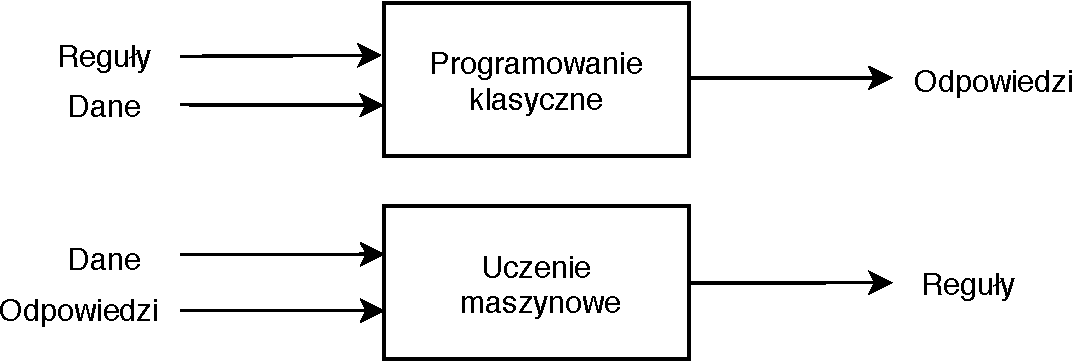
\includegraphics[width=10cm]{uczenie_maszynowe.pdf}
	\centering
	\caption{Uczenie maszynowe: nowy model programowania}
	\label{fig:uczenie_maszynowe}
\end{figure}
\\

Podsumowując, system uczenia maszynowego jest trenowany, a nie programowany w sposób jawny. Celem programisty jest przedstawienie mu odpowiedniej dużej ilości przykładów wyników, tak by sam system określił ich statystyczną strukturę, co w dalszej części pozwoli na ustalenie reguł umożliwiających automatyzację całego procesu. Ważne, by podkreślić tutaj znaczenie danych wejściowych, które to często określa się terminem \textit{Big Data}\cite{big_data}.

\section{Big Data}

Popularyzację tego terminu przypisuję się do wykładu autorstwa Johna Mashey'a\cite{mashey} jaki wygłosił w 1998 roku. Zauważył on, że wraz ze spadkiem cen nośników do przechowywania i gromadzenia danych, ilość zbieranych przez ludzkość informacji wzrasta z każdym rokiem. Co więcej, ilość tych danych sprawia, że ich analiza przestała być możliwa do realizacja w sposób inny niż automatyczny. Za kryterium, czy dany zbiór informacji można określić jako Big Data, często przywołuje się te podane przez Douglasa Laney'ego\cite{laney} i określane mianem \textit{3V}, które to rozwija się jako rozmiar(ang. \textit{volume}), różnorodność(ang. \textit{variety}) i prędkość (ang. \textit{velocity}). Oznaczają one kolejno:
\begin{itemize}
	\item \textbf{rozmiar} - dane są zbyt duże by mieściły się na standardowych dyskach twardych,
	\item \textbf{różnorodność} - dane pochodzą z różnych źródeł, są niejednorodne i słabo ustrukturyzowane,
	\item \textbf{prędkość} - tempo napływu nowych danych jest znaczące, co w rezultacie utrudnia ich analizowanie.
\\
\end{itemize}

Jednym z kluczowych zjawisk przyczyniającym się do procesu nagłego przyrostu ilości i źródeł danych jest Internet przedmiotów (ang. \textit{Internet of Things}\cite{iot}). Według tej koncepcji, różnego typu urządzenia osadzone w urządzeniach codziennego użytku(np. odkurzacze, żarówki, instalacje grzewcze), czy też w maszynach przemysłowych, zbierają dane o otoczeniu, czy samym procesie w którym uczestniczą, a ponadto mają możliwość komunikacji pomiędzy sobą, ale również z jednostką centralną jeśli taka występuje. Wprowadza to nowy wymiar w możliwościach automatyzacji procesów i tworzy nową przestrzeń do tworzenia się złożonych, inteligentnych systemów.

\section{Rodzaje systemów uczenia maszynowego}

Istnieje wiele metod podziału uczenia maszynowego na kategorię. Jedną z najpopularniejszych jest podział ze względu na sposób uczenia się oraz zadanie do wykonania\cite{python_ml}:
\begin{itemize}
	\item Uczenie nadzorowane:
	\begin{itemize}
		\item klasyfikacja,
		\item regresja.
	\end{itemize}
	\item Uczenie nienadzorowane:
	\begin{itemize}
		\item klasteryzacja,
		\item redukcja wymiarowości,
		\item uczenie przy użyciu reguł asocjacyjnych.
	\end{itemize}
	\item Uczenie ze wzmocnieniem.\\
\end{itemize}

W uczeniu z nadzorem(ang. \textit{supervised learning}), którym zajmę się w poniżej pracy, dane trenujące przekazane algorytmowi zawierają dołączone do nich etykiety, czyli rozwiązania problemu. Celem algorytmu jest stworzenie funkcji(nazywanej też hipotezą\cite{cichosz}), która będzie maksymalizować swoją skuteczność względem zadanych kryteriów.
\\

Na zbiór uczący $Z_{u}$ składa się zbiór $n$ wektorów, gdzie każdy z nich opisuje pojedynczy obiekt(patrz wzór \ref{eqn:zbiot_t}):
\begin{equation}
	Z_{u}=\left \{(x_{1},y_{1}),...,(x_{n},y_{n})\right \}
	\label{eqn:zbiot_t}
\end{equation}
I tak w powyższym równaniu\ref{eqn:zbiot_t}) $i$-ty wektor oznaczony byłby jako $x_{i}$ i odpowiadałaby mu etykieta oznaczona jako $y_{i}$. W zależności od typu danych przechowywanych pod etykietą będziemy mieć do czynienia z zadaniem klasyfikacji(etykieta należy do skończonego i przeliczalnego zbioru) lub regresji(wartości przyjmowane przez etykietę należą do przestrzeni ciągłej). Ważne żeby dodać że na wektor $x_{i}$ może składać się $m$-liczb, gdzie każdą z tych liczb będziemy nazywać atrybutem lub cechą danego wektora(patrz wzór \ref{eqn:wek}):
\begin{equation}
	x_{i} = \left \{ x_{1,m}, ..., x_{i,m} \right \}
	\label{eqn:wek}
\end{equation}
Etykietą $y_{i}$, w tym rozumowaniu, oznaczamy prawdziwą wartość funkcji, którą to chcemy by nasz algorytm odwzorował. Algorytm ten, nazywamy również modelem i opisujemy go jako następującą funkcję $f$(patrz wzór \ref{eqn:func_f}):
\begin{equation}
	f(x): x \in X \mapsto y \in Y
	\label{eqn:func_f}
\end{equation}
Jak widać zadaniem powyższej funkcji jest przyporządkowanie wektorom wejściowym etykiet. Jej skuteczność jest mierzona przy użyciu wybranej przez nas metryki na zbiorze testowym. Zbiór testowy musi posiadać tą samą strukturę co zbiór trenujący. Można traktować metrykę $M$ jako funkcję wyższego rzędu, której pierwszym argumentem jest sam model $f$, a drugim zbiór testowy $Z_{t}$. Dziedziną metryki jest zazwyczaj podzbiór liczb rzeczywistych z zakresu od 0 do 1(patrz wzór \ref{eqn:metric})
\begin{equation}
	M(f, Z_{t}): (f, Z_{t}) \mapsto m \in [0, 1]
	\label{eqn:metric}
\end{equation}
Przykładem metryk stosowanych w uczeniu maszynowym są między innymi dokładność, czułość, precyzja, a także miara \textit{F} (ang. \textit{F-score}), które
omówione zostały szczegółowo w dalszej części rozdziału.
\\

\section{Problem przeuczania, niedouczania}

Wykorzystanie osobnego zbioru do badania jakości modelu w uczeniu nadzorowanym związane jest bezpośrednio z takimi problemami jak nadmierne dopasowanie, przeuczenia(ang. \textit{overfitting}) oraz niedouczenie (ang. \textit{underfitting})\cite{hands_on}. Zadaniem, które dobrze nadaje się do graficznej ilustracji powyższych problemów jest regresja liniowa. Jak już zostało opisane powyżej w problemie tym, etykiety
przykładów są liczbami należącymi do przestrzeni ciągłej, a zadaniem algorytmu jest wyznaczenie funkcji f(patrz wzór \ref{eqn:reg}):
\begin{equation}
	f(x): x \mapsto y \in \mathbb{R}
	\label{eqn:reg}
\end{equation}
Dodatkowo dla lepszej interpretacji graficznej każdy wektor w przestrzeni $x$ będzie posiadał tylko jedną cechę. Przykład prawidłowego dopasowania wygląda następująco(patrz rysunek \ref{fig:probki}):

\begin{figure}[h!]
	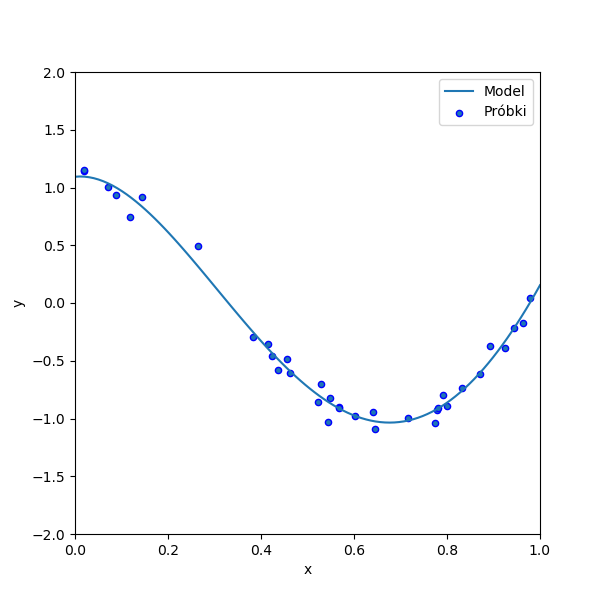
\includegraphics[width=6cm]{good.png}
	\centering
	\caption{Przykład prawidłowego dopasowania}
	\label{fig:probki}
\end{figure}

Problem nadmiernego dopasowania cechuje się tym, że taki model zbyt mocno generuje charakterystykę dla danych trenujących, zawierając w niej również występujące tam szumy(patrz rysunek \ref{fig:overfitting}):

\begin{figure}[h!]
	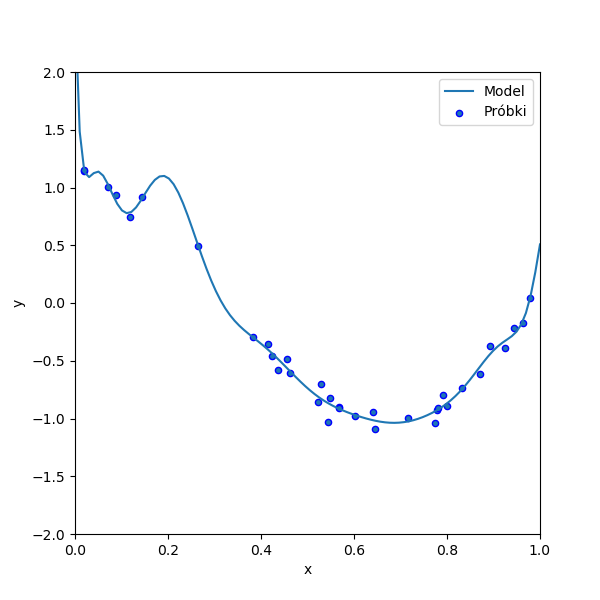
\includegraphics[width=6cm]{overfitting.png}
	\centering
	\caption{Przykład nadmiernego dopasowania}
	\label{fig:overfitting}
\end{figure}

Odwrotnym problem jest problem niedouczenia. Występuję on na przykład wtedy, kiedy zastosujemy zbyt prosty model w stosunku do poziomu skomplikowania zbioru danych. Wynik takiej operacji widoczny jest na rysunku \ref{fig:underfitting} 

\begin{figure}[h!]
	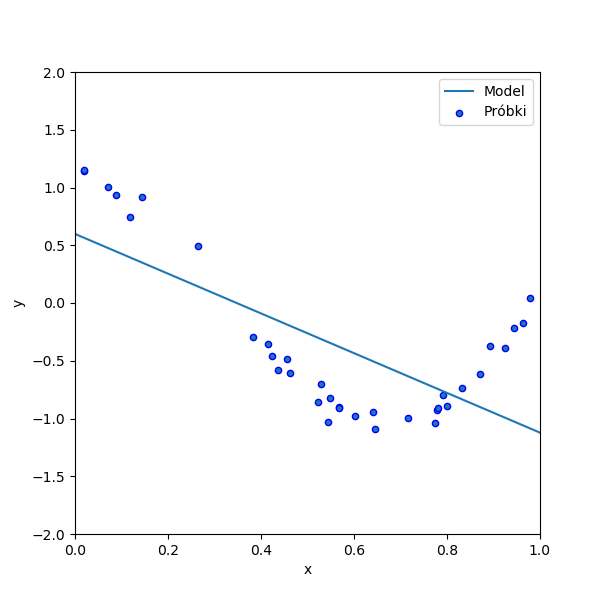
\includegraphics[width=6cm]{underfitting.png}
	\centering
	\caption{Przykład niedostatecznego dopasowania}
	\label{fig:underfitting}
\end{figure}

\section{Zadanie klasyfikacji binarnej}

W niniejszej pracy będę zajmował się zadaniem należącym do problemów klasyfikacji binarnej, czyli takiej w której przestrzeń etykiet ogranicza się do dwóch elementów(patrz wzór \ref{eqn:zbiot_y}):
\begin{equation}
	y=\left \{0, 1\right \}
	\label{eqn:zbiot_y}
\end{equation}
Klasy $0$ i $1$ w powyższym wzorze\ref{eqn:zbiot_y} są przykładowe i bardziej niż ich wartość interesuje Nas liczność zbioru $y$. Tym samym mając zdefiniowaną przestrzeń możliwych wartości modelu można zdefiniować szereg miar, które są wykorzystywane do oceny jego wyników. Podstawowym elementem zadania ewaluacji modelu w zadaniu klasyfikacji binarnej jest macierz, tablica błędów widoczna w tabeli \ref{tab:macierz_bledow}. Do jej skonstruowania potrzebujemy oczywiście przetestować działanie naszego modelu na zbiorze testowym $Z_{t}$. Poszczególnym reprezentantom tego zbioru, przypisywane są pozytywne lub negatywne etykiety, teraz w zależności od tego czy dany element zbioru $x$ był faktycznie pozytywny czy negatywny można go wpisać w macierz błędów \ref{tab:macierz_bledow}.
\begin{table}[h!]
	\centering
	\begin{tabular}{c|c|c|}
		\cline{2-3}
		&
		\textbf{\begin{tabular}[c]{@{}c@{}}Klasyfikacja \\ pozytywna\end{tabular}} &
		\textbf{\begin{tabular}[c]{@{}c@{}}Klasyfikacja \\ negatywna\end{tabular}} \\ \hline
		\multicolumn{1}{|c|}{\textbf{\begin{tabular}[c]{@{}c@{}}Stan \\ pozytywny\end{tabular}}} &
		\begin{tabular}[c]{@{}c@{}}Prawdziwie dodatnia\\ (ang. \textit{true positive}, TP)\end{tabular} &
		\begin{tabular}[c]{@{}c@{}}Fałszywie ujemna\\ (ang. \textit{false negative}, FN)\end{tabular} \\ \hline
		\multicolumn{1}{|c|}{\textbf{\begin{tabular}[c]{@{}c@{}}Stan \\ negatywny\end{tabular}}} &
		\begin{tabular}[c]{@{}c@{}}Fałszywie dodatnia\\ (ang. \textit{false positive}, FP)\end{tabular} &
		\begin{tabular}[c]{@{}c@{}}Prawdziwie ujemna\\ (ang. \textit{true negative}, TN)\end{tabular} \\ \hline
	\end{tabular}
	\caption{Tablica pomyłek, możliwe wyniki klasyfikacji binarnej}
	\label{tab:macierz_bledow}
\end{table}

\section{Ewaluacja modelu - Miary jakości}

Korzystając z opisanej powyżej macierzy błędów \ref{tab:macierz_bledow} w łatwy sposób można przedstawić definicję szeregu miar do oceny modelu, z których to skorzystałem w niniejszej pracy:
\begin{itemize}
	\item \textbf{Dokładność} - procent poprawnych klasyfikacji, opisanych wzorem \ref{eqn:acc}:
		\begin{equation}
			\mathbf{accuracy} = \frac{TP + TN}{TP + TN + FP + FN}
			\label{eqn:acc}
		\end{equation}
	\item \textbf{Czułość} - stosunek prawidłowych wyników pozytywnych do sumy prawidłowych wyników pozytywnych oraz błędnych wyników negatywnych, który można rozumieć jako zdolność modelu do poprawnego etykietowania(patrz wzór \ref{eqn:rec}),
		\begin{equation}
			\mathbf{recall} = \frac{TP}{TP + FN}
			\label{eqn:rec}
		\end{equation}
	\item \textbf{Precyzja} - stosunek prawidłowych wyników pozytywnych do sumy prawidłowych wyników pozytywnych oraz błędnych wyników pozytywnych, który można rozumieć jako zdolność modelu do niepoprawnej klasyfikacji próbek negatywnych jako pozytywne(patrz wzór \ref{eqn:prec}),
		\begin{equation}
			\mathbf{precision} = \frac{TP}{TP + FP}
			\label{eqn:prec}
		\end{equation}
	\item \textbf{miara \textit{F}} - będąca średnią ważoną z czułości i precyzji(patrz wzór \ref{eqn:fscore}).
		\begin{equation}
			\mathbf{F1}= \frac{2 * precision * recall}{precision + recall}
			\label{eqn:fscore}
		\end{equation}
\end{itemize}

\section{Splotowe sieci neuronowe}

Splotowe, inaczej konwolucyjne, sieci neuronowe (ang. \textit{CNN - convolutional neural networks}) stanowią wynik badań nad korą wzrokową i od 1980 roku są używane w zadaniach rozpoznawania obrazów\cite{hands_on}. Podstawową różnicą w stosunku do sieci neuronowych jest stosowanie wielowymiarowej operacji splotu, realizowanej za pomocą szeregu filtrów, których to parametry dobierane są podczas trenowania sieci. Pozwala to siecią konwolucyjnym na nie przetwarzanie obrazów piksel po pikselu, a raczej poprzez zauważanie ogólnych cech obrazu i budowaniu z nich nowych struktur. \\

W analizie matematycznej operacją splotu(reprezentowana jako $*$) dwóch funkcji $f$ i $g$, jest trzecia funkcja $s$, patrz wzór \ref{eqn:splot}:
\begin{equation}
	\begin{split}
		s(t) = (f * g)(t) & = \int_{-\infty}^{\infty}f(\tau)g(t-\tau)d\tau =\\
						  & =\int_{-\infty}^{\infty}f(t-\tau)g(\tau)d\tau
	\end{split}
	\label{eqn:splot}
\end{equation}
, a w przypadku operacji dyskretnych, patrz wzór \ref{eqn:splot_d}:
\begin{equation}
	s(t)=(f*g)(t)=\sum_{\tau = -\infty}^{\infty}f(\tau)(g-\tau)
	\label{eqn:splot_d}
\end{equation}
W literaturze opisującej sieci neuronowych przyjęło się określać $f(\tau)$ jako wejście, $g(t - \tau)$ jako jądro lub filtr(z ang. \textit{kernel}, \textit{filter}), a wynik samej operacji jako mapę atrybutów lub aktywacji (z ang. \textit{feature map}, \textit{activation map})\cite{piczak}. Zadanie dla typowego problemu klasyfikacji obrazów, operującego na dwuwymiarowym obrazie wejściowym $M$ przy pomocy filtra $K$ z założeniem wykorzystania wielowymiarowego splotu $S(i, j)$, można sformułować następująco \ref{eqn:splot_mk}:
\begin{equation}
	\begin{split}
	S(i, j) & = (M*K)(i,j)=\sum_{k}^{}\sum_{l}^{}M(k,l)K(i-k,j-l) \\
		    & = (K*M)(i,j)=\sum_{k}^{}\sum_{l}^{}M(i-k,j-l)K(k,l)
	\end{split}
	\label{eqn:splot_mk}
\end{equation}

\section{Uczenie głębokie}

Budowa sieci splotowych, a dokładnie fakt, że nie wymagały one połączeń pomiędzy wszystkimi neuronami w każdej z warstw oraz fakt, że zastosowanie operacji splotu, pozwala na zmniejszenie wymiarów zdjęcia pozwoliło budować sieci o większej ilości warstw ukrytych \cite{python_ml}. Za pierwszą pracę z stosującą uczenie głębokie(funkcje splotu, wsteczną propagację) uważa się tą 1989 roku, której autorzy stworzyli model rozpoznający kody pocztowe\cite{lecun}. Sam model okazał się sukcesem, problemem był jednak czas uczenia - $\sim$3 dni. Z racji jednak że w ostatnim czasie moc obliczeniowa komputerów wzrosła kilkukrotnie, oraz dodatkowo same zbiory danych zwiększyły swoje rozmiary i jakość - uczenie głębokie staje coraz popularniejsze\cite{hands_on}.

























